\documentclass[12pt,a4paper,twoside]{report}
\usepackage[italian]{babel}
\usepackage{newlfont}
\usepackage{color}
\textwidth=450pt\oddsidemargin=0pt

% INIZIO HEADER INSERITI DA ME, DA CUI HO TOLTO GLI HEADER CHE SI RIPETONO

%\documentclass[12pt,a4paper]{article}
%\usepackage[utf8]{inputenc}
\usepackage{titling}
\usepackage[backend=bibtex,
			style=numeric,
			sorting=none
			]{biblatex}
\addbibresource{bibliography.bib} %Import the bibliography file
%\setlength{\droptitle}{-2cm}% change title position
\usepackage{amsmath}
%\usepackage{amsfonts}
\usepackage{amssymb}
%\usepackage[T1]{fontenc}
%\usepackage{multirow}
%\usepackage{array}
%\newcolumntype{P}[1]{>{\centering\arraybackslash}p{#1}}
%\newcolumntype{M}[1]{>{\centering\arraybackslash}m{#1}}
\usepackage{graphicx}
%\usepackage{siunitx}
\usepackage{hyperref}
\usepackage{float}
\usepackage[top=1.7in,left=1in,right=1in]{geometry}
%\usepackage{listings}
%\usepackage{circuitikz}
%\usepackage{subcaption}
%\usepackage{tabularx}
\hypersetup{
	colorlinks,
	citecolor=black,
	filecolor=black,
	linkcolor=black,
	urlcolor=black
}
%\renewcommand{\lstlistingname}{Code}
%\renewcommand{\lstlistlistingname}{List of Code}
%\lstdefinestyle{chstyle}{
	%	backgroundcolor=\color{gray!12},
	%	basicstyle=\ttfamily\small,
	%	commentstyle=\color{green!60!black},
	%	keywordstyle=\color{magenta},
	%	stringstyle=\color{blue!50!red},
	%	showstringspaces=false,
	%	%captionpos=b,
	%	numbers=left,
	%	numberstyle=\footnotesize\color{gray},
	%	numbersep=10pt,
	%	%stepnumber=2,
	%	tabsize=2,
	%	frame=L,
	%	framerule=1pt,
	%	rulecolor=\color{red},
	%	breaklines=true,
	%	inputpath=code
	%}
%\renewmenumacro{\directory}{pathswithfolder} % default: path
%\renewmenumacro{\keys}{shadowedroundedkeys} % default: roundedkeys
%\setlength{\arrayrulewidth}{1.0pt}
%\renewcommand{\arraystretch}{1}
\usepackage{mathcomp}

%\usepackage{fontspec}
%\setmainfont{Calibri}

\usepackage{fancyhdr}
\pagestyle{fancy}
%\renewcommand{\chaptermark}[1]{\markboth{\MakeUppercase{\chaptername\ \thechapter.\ #1}}{}}
\renewcommand{\chaptermark}[1]{\markboth{\MakeUppercase{CAP.\ \thechapter\ --\ #1}}{}}
\setlength{\headwidth}{13cm}
\fancyhead{} % clear all header fields
\fancyhead[LO]{\footnotesize \textsl{\rightmark}}
\fancyhead[RE]{\footnotesize \textsl{\leftmark}}
\fancyhead[LE,RO]{\footnotesize \thepage}
\fancyfoot{} % clear all footer fields
\renewcommand{\headrulewidth}{0.3pt}

% è già di default interlinea singola
\usepackage{setspace}

%\usepackage[font=it]{caption}
%\usepackage{indentfirst}

% FINE HEADER INSERITI DA ME

\begin{document}
	\begin{titlepage}
		\begin{center}
			{{\Large{\textsc{Alma Mater Studiorum $\cdot$ Universit\`a di Bologna}}}} 
			\rule[0.1cm]{15.8cm}{0.1mm}
			\rule[0.5cm]{15.8cm}{0.6mm}
			\\\vspace{3mm}
			
			{\small{\bf Scuola di Scienze \\ 
					Dipartimento di Fisica e Astronomia\\
					Corso di Laurea in Fisica}}
			
		\end{center}
		
		\vspace{23mm}
		
		\begin{center}\textcolor{red}{
				%
				% INSERIRE IL TITOLO DELLA TESI
				%
				{\LARGE{\bf TITOLO TESI}}\\
		}\end{center}
		
		\vspace{50mm} \par \noindent
		
		\begin{minipage}[t]{0.47\textwidth}
			%
			% INSERIRE IL NOME DEL RELATORE CON IL RELATIVO TITOLO DI DOTTORE O PROFESSORE
			%
			{\large{\bf Relatore: \vspace{2mm}\\\textcolor{red}{
						Prof./Dott. Nome Cognome}\\\\
					%
					% INSERIRE IL NOME DEL CORRELATORE CON IL RELATIVO TITOLO DI DOTTORE O PROFESSORE
					%
					% SE NON AVETE UN CORRELATORE CANCELLATE LE PROSSIME 3 RIGHE
					%
					\textcolor{red}{
						\bf Correlatore: (eventuale)
						\vspace{2mm}\\
						Prof./Dott. Nome Cognome\\\\}}}
		\end{minipage}
		%
		\hfill
		%
		\begin{minipage}[t]{0.47\textwidth}\raggedleft {
				{\large{\bf Presentata da:
						\vspace{2mm}\\
						Simone Pasquini}}}
		\end{minipage}
		
		\vspace{40mm}
		
		\begin{center}
			Anno Accademico { 2023/2024}
		\end{center}
		
	\end{titlepage}
	\newpage
	\newgeometry{top=4cm,bottom=4cm,left=4cm,right=4cm}
	\doublespacing % Also singlespacing, onehalfspacing 
	\chapter*{Sommario}
		Questo è l'inizio del sommario.
	\newpage
	\tableofcontents
	\newpage
	\addcontentsline{toc}{chapter}{Introduzione}
	\chapter*{Introduzione}
		Questo è l'inizio dell'introduzione.
	\newpage
	\addcontentsline{toc}{chapter}{Conclusioni}
	
	\chapter{Terapie oncologiche e radiazioni ionizzanti}
	\section{Incidenza tumorale nel mondo}
	Tra le principali cause di morte per la popolazione mondiale emerge la contrazione di neoplasie (o tumori). Un tumore è una patologia legata al mancato funzionamento del ciclo cellulare. Le cellule tumorali, per via di mutazioni genetiche che sfuggono ai meccanismi di controllo che regolano la proliferazione cellulare, iniziano a dividersi in modo eccessivo formando delle masse anomale, chiamate tumori, che talvolta possono invadere altri tessuti dell'organismo ostacolandone le funzioni vitali, in un processo chiamato metastasi. In quest'ultimo caso si parla di tumore maligno o cancro.
		
	Attualmente, è possibile prevenire fino al $50\%$ di tumori evitando fattori di rischio e implementando strategie di prevenzione già esistenti (cita
	%https://www.who.int/news-room/fact-sheets/detail/c+ancer
	), anche se ciò dipende dalla tempestività delle diagnosi, dalla tipologia delle cure e dal tipo di tumore. Si stima che nei Paesi industrializzati\footnote{Si fa riferimento ai Paesi OCSE (Organizzazione per la Cooperazione e lo Sviluppo Economico).}, nel $2021$, il cancro è la seconda causa di morte (causando il $21\%$ dei decessi totali), preceduto dalle malattie cardiovascolari (cita %https://www.oecd-ilibrary.org/docserver/7a7afb35-en.pdf?expires=1709230714&id=id&accname=guest&checksum=FBEABF3EDA6F2040465BB27356B8D68B
	). Sebbene il tasso di mortalità sia sceso sin dal $2000$, a livello mondiale il numero di casi diagnosticati di cancro (nel $2022$) attesta a quasi $20.0$ milioni\footnote{Negli ultimi dieci anni il numero di casi di tumore è aumentato di anno in anno, soprattutto a causa dell'invecchiamento progressivo della popolazione (cita
	%https://www.iss.it/-/tumori-in-aumento-le-diagnosi-in-europa-anche-per-effetto-dell-invecchiamento-demografico
	), ma nel biennio $2020$-$2021$ il trend è cambiato a causa della pandemia di COVID-$19$, che ha precluso l'accesso a screening oncologici (nel periodo gennaio--ottobre $2020$ vi è stato un calo del $37.3\%$ di test diagnostici rispetto al periodo pre-pandemico) (cita
	%https://www.ncbi.nlm.nih.gov/pmc/articles/PMC9807424/
	). Ciò potrebbe rivelarsi fatale nel medio-lungo termine causando un aumento dei tassi di incidenza e mortalità (cita
	%https://doi.org/10.1787/ae3016b9-en
	).} (pari al $2.5\tcperthousand$ della popolazione totale (citare %https://data.unicef.org/resources/data_explorer/unicef_f/?ag=UNICEF&df=GLOBAL_DATAFLOW&ver=1.0&dq=WORLD.DM_POP_TOT.&startPeriod=2022&endPeriod=2022
	)), di cui il $48.8\%$ hanno portato alla morte del paziente (citare
	%https://gco.iarc.who.int/en
	). Inoltre, i tassi di mortalità dovuti alle patologie tumorali sono strettamente dipendenti dall'indice di sviluppo dei Paesi (ISU), infatti da un tasso di mortalità del $39.2\%$ dei Paesi con ISU molto alto, si sale sino al $67.1\%$ dei Paesi con basso ISU (cita
	%https://gco.iarc.who.int/today/en/dataviz/bars?mode=population&key=total&group_populations=0&types=0_1&sort_by=value1&populations=900_981_982_983_984&multiple_populations=1&values_position=out&cancers_h=39&include_nmsc=1&age_end=17
	).
	
	Altri fattori rendono i tassi di incidenza e mortalità per patologie tumorali ulteriormente disuniformi, quali il sesso e l'età. A livello globale, l'incidenza di cancro negli uomini è più alta rispetto a quella delle donne dell'$8.0\%$ (cita
	%https://gco.iarc.who.int/media/globocan/factsheets/cancers/39-all-cancers-fact-sheet.pdf
	), dovuta anche al fatto che i primi si espongono maggiormente a fattori di rischio quali fumo e consumo di alcol. Inoltre, il $58\%$ di tumori viene diagnosticato nelle persone con più di 65 anni (cita
	%https://www.cdc.gov/cancer/uscs/about/data-briefs/no29-USCS-highlights-2019-incidence.htm
	).
	
	Sebbene i dati sopra citati testimonino la gravità delle patologie oncologiche, è indubbio che il progresso della scienza degli ultimi anni abbia permesso un notevole sviluppo nell'efficacia dei trattamenti oncologici: nel decennio $2010$--$2020$, il numero di persone che sopravvive dopo una diagnosi di cancro aumenta approssimativamente del $3\%$ in Paesi come l'Italia, gli Stati Uniti d'America, il Regno Unito e la Svizzera (cita
	%https://www.ncbi.nlm.nih.gov/pmc/articles/PMC5807846/pdf/12885_2018_Article_4053.pdf
	).
	
	\section{Terapie oncologiche}
	Il trattamento di un tumore avviene in molti modi differenti e varia in base al tipo di cancro, il suo stadio di avanzamento e dagli obiettivi che si intendono raggiungere al termine dei trattamenti. Oggigiorno, le terapie oncologiche si distinguono in locali (o regionali) e generali (o sistemiche), in base all'estensione del tumore che colpisce il paziente. Al primo gruppo appartengono terapie come la chirurgia, la radioterapia e l'adroterapia, mentre al secondo afferiscono la chemioterapia e l'immunoterapia. Tali tecniche, proprio per la loro diversità, sono spesso utilizzate in maniera complementare per aumentare l'efficacia dei trattamenti clinici. Per pianificare il trattamento più adeguato al fronte di una certa patologia oncologica, si introduce il concetto di stadiazione, che è un modo di descrivere in maniera schematica, rigorosa e standardizzata la grandezza di un tumore e la sua diffusione al di fuori della sede originale (cita
	%https://www.airc.it/cancro/affronta-la-malattia/la-fase-della-diagnosi/stadiazione
	). Le informazioni tipiche della stadiazione includono la collocazione del tumore, la sua estensione e se si è diffuso in parti del corpo differenti. Infatti, come già accennato, le cellule tumorali si moltiplicano in modo incontrollato andando a occupare (per mezzo del sistema linfatico o sanguigno) organi e tessuti distanti dalla sede di sviluppo originaria, attraverso un fenomeno chiamato metastatizzazione. Chiaramente, ciascuna terapia possiede effetti collaterali correlati all'azione distruttiva che si impiega per debellare la malattia oncologica.
	
	Se il tumore ha raggiunto un'estensione tale da formare metastasi, si scelgono trattamenti sistemici in modo che si possa debellare o, quantomeno, contenere la malattia oncologica. La chemioterapia consiste nella somministrazione di uno o più farmaci citotossici (o antiblastici) capaci di aggredire le cellule cancerose (cita
	%https://www.aimac.it/libretti-tumore/chemioterapia/che-cos-e-la-chemioterapia
	), mentre nell'immunoterapia si tenta di istruire il sistema immunitario affinché riconosca ed elimini gli oncogeni, i geni modificati che causano il cancro.
	
	Qualora il tumore fosse localizzato, ben raggiungibile dall'esterno e sufficientemente lontano da organi vitali, si ricorre a operazioni chirurgiche, con le quali si asporta la massa tumorale dal corpo del paziente. Prima o dopo l'operazione chirurgica, si procede con tecniche radioterapiche, adroterapiche o chemioterapiche in base alle necessità. Ad esempio, nella radioterapia neoadiuvante il trattamento radioterapico viene effettuato prima dell'intervento chirurgico, mentre nella radiochemioterapia concomitante si eseguono sessioni di chemioterapia e radioterapia a seguito dell'operazione chirurgica (cita
	%https://www.aimac.it/libretti-tumore/radioterapia/perche-si-attua-la-radioterapia
	). In generale, la commistione di suddette tecniche consente di rimuovere tracce di cellule tumorali, evitandone eventuali proliferazioni successive.
	
	Nel caso in la massa tumorale non sia rimovibile attraverso un'operazione chirurgica a causa della sua localizzazione anatomica (è il caso di neoplasie legate a organi la cui rimozione sarebbe troppo invalidante per il paziente (cita
	%https://web.infn.it/foot/
	)), si preferisce ricorrere alla radioterapia e all'adroterapia. Pur non essendo invasive come la chirurgia, tali tecniche permettono di danneggiare specifici tessuti biologici malati utilizzando radiazione ionizzante, composta da fasci di fotoni ed elettroni in radioterapia e da particelle adroniche (come protoni, neutroni e ioni) in adroterapia (si veda \hyperref[fig:simulation]{Fig. 1.1}). In particolare, lo scopo di entrambi i trattamenti è quello di depositare una quantità di energia (detta "dose") capace di provocare un danno biologico tale da inibire la crescita del tumore con effetti collaterali minimi (cita
	%rivista asimmetrie, DOI 10.23801/asimmetrie.2023.35.03
	). Sebbene sembrino molto simili, la radioterapia e l'adroterapia presentano caratteristiche fisiche e radiobiologiche molto differenti, i cui dettagli verranno evidenziati nel prosieguo. Mentre un fascio radioterapico rilascia la dose in una regione piuttosto ampia, aumentando il rischio di distruggere cellule sane situate prima e dopo il tumore, le particelle adroniche irradiano una grande quantità di energia in uno spazio molto limitato, attraverso il caratteristico picco di Bragg (BP). Pertanto, visto che l'adroterapia permette di definire in modo molto più preciso la regione da irradiare (cita
	%https://web.infn.it/foot/
	), il suo obiettivo non è solo quello di distruggere più efficacemente porzioni di cellule tumorali, ma anche quello di minimizzare i danni a carico dei tessuti sani circostanti (cita
	%https://fondazionecnao.it/adroterapia/cos-e-l-adroterapia
	), al fine di qualità della vita del paziente.
	
	\begin{figure}[H]
		\centering
		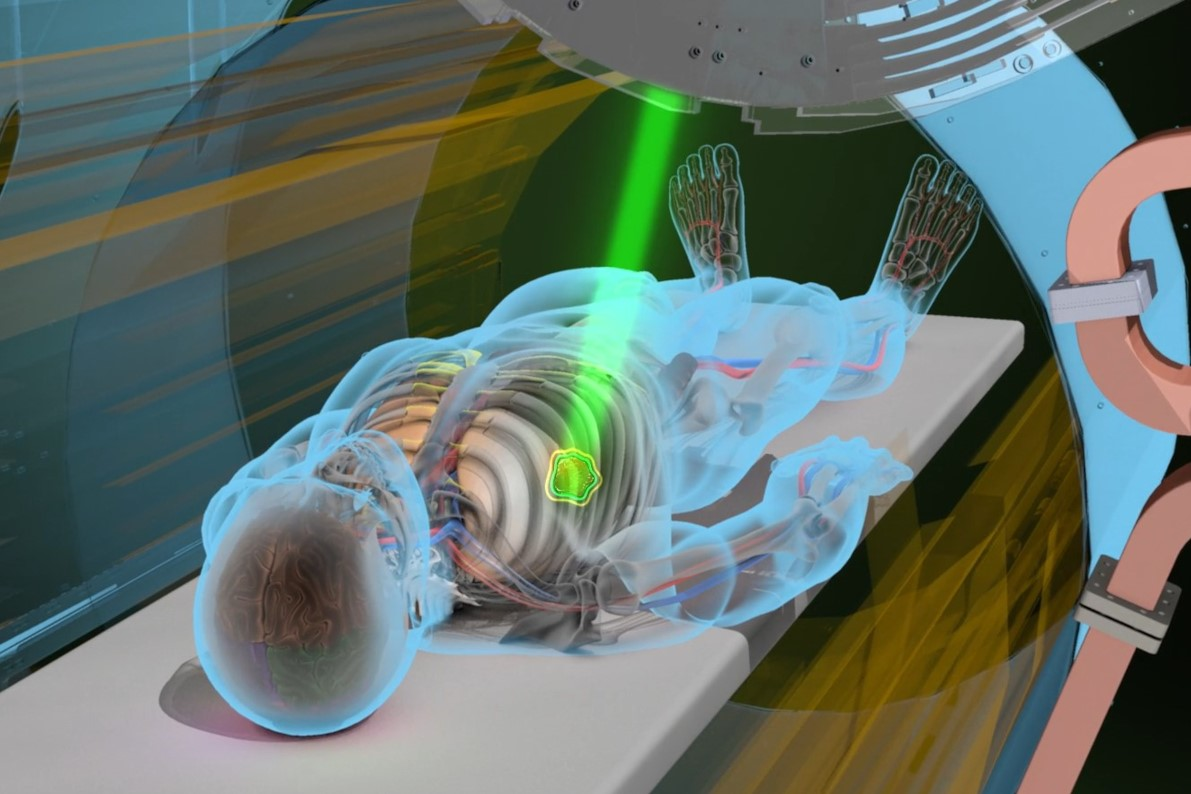
\includegraphics[width=0.9\linewidth]{images/simulation.jpg}
		\caption{Simulazione di un irraggiamento radioterapico o adroterapico sul corpo di un paziente (cita
			%https://www.youtube.com/watch?v=Uu261OEf3Pg
			).}
		\label{fig:simulation}
	\end{figure}
	
	Sebbene l'adroterapia sia complessivamente più efficace rispetto alla radioterapia nella distruzione di cellule tumorali e nella salvaguardia dei tessuti sani, è un trattamento relativamente recente (si veda \hyperref[storia_adroterapia]{Sez. 1.2}), dunque meno sviluppato e più costoso rispetto alla radioterapia. Infatti, oggi non esiste una teoria analitica che sia in grado di spiegare i processi nucleari che intercorrono tra le particelle adroniche e i nuclei del corpo umano (cita
	%FOOT CDR
	), quindi, prima di poter applicare trattamenti medici efficaci e sicuri, si rendono necessarie numerosissime misure sperimentali (una buona parte delle quali sono tuttora fornite dall'esperimento FOOT) in grado di colmare tali lacune (cita
	%https://web.infn.it/foot/
	). Per questo motivo, il settore di ricerca adroterapico è molto attivo e coinvolge un crogiolo culturale di fisici, medici, biologi che studiano gli effetti della frammentazione nucleare sulle cellule umane, analizzabili solo mediante un approccio interdisciplinare.
	
	L'adroterapia, però, non appartiene esclusivamente all'ambito della sperimentazione, ma costituisce una realtà interazionale nella cura dei tumori a tutti gli effetti. Infatti, alla fine del $2023$ quasi $410000$ pazienti hanno effettuato trattamenti adroterapici a livello globale (di cui $350000$ con protoni, $56000$ con ioni carbonio e $3500$ con elio, pioni e altre particelle), un numero tre volte maggiore di quello emerso a fine $2014$ (cita
	%https://ptcog.site/
	). Pur essendo tali numeri incoraggianti, è necessario continuare a investire risorse nella ricerca in modo che esperimenti della caratura di FOOT possano rendere l'adroterapia un trattamento più diffuso e accessibile a tutti.
	

%	l’idea di usare i protoni per il trattamento del cancro fu proposta per la prima volta nel 1946 L’adroterapia è un forma molto avanzata di radioterapia. La radioterapia, da sola o associata a chirurgia e/o a chemioterapia, migliora il controllo locale in diverse patologie tumorali. Inoltre, la natura non invasiva delle radiazioni rappresenta una valida alternativa per quei tumori non aggredibili chirurgicamente perché localizzati in sedi anatomiche complicate da organi vitali o deputati a funzioni la cui asportazione sarebbe troppo invalidante per il paziente.
	
%	La forza dell’adroterapia è nelle proprietà fisiche e radiobiologiche uniche delle particelle cariche (adroni): esse possono penetrare nei tessuti con poca diffusione e depositare la massima energia appena prima di fermarsi. Ciò consente di definire in modo molto preciso la region da irradiare. La caratteristica forma a picco del deposito di energia è chiamata picco di Bragg ed è diventata il simbolo dell’adroterapia.

% dire che FOOT L'esperimento FOOT unisce laboratori giapponesi, tedeschi e italiani al ne di raccogliere dati fondamentali per migliorare la conoscenza delle interazioni tra i fasci adronici e il materiale

	\section{Storia dell'adroterapia}\label{storia_adroterapia}
	
	
	
			
	
	\chapter*{Conclusioni}
		Let's cite! Einstein's journal paper \cite{einstein} and Dirac's book \cite{dirac} are physics-related items.
	\newpage	
	\printbibliography[
		heading=bibintoc,
		title={Bibliografia}
		]
		 	
\end{document}

